\documentclass[border=10pt]{standalone}
\usepackage{pgfplots}
\pgfplotsset{width=7cm,compat=1.8}
\pgfplotsset{
    colormap/outer/.style={
        colormap=
            {outer}{
            rgb255(0cm)=(0,128,192);
            rgb255(1cm)=(0,64,128);
            }
    },
    colormap/outer,
    colormap/inner/.style={
        colormap={inner}{
            rgb255(0cm)=(0,64,128);
            rgb255(1cm)=(180,220,255);
        }
    },
    colormap/inner
}
\begin{document}
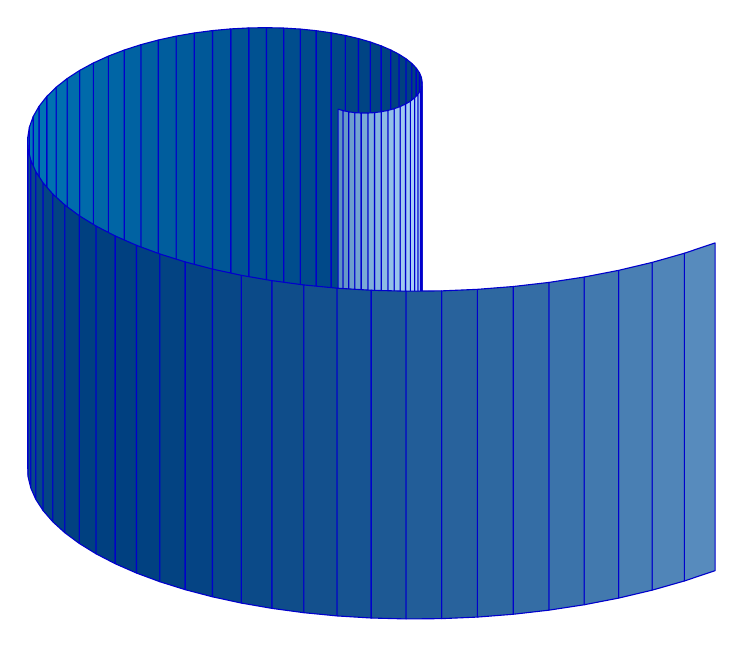
\begin{tikzpicture}
  \begin{axis}[
      hide axis,
      axis equal image,
      z buffer=sort,
      view={40}{25},
      width=15cm
    ]
    \addplot3 [
      surf,
      domain=0:2*pi,
      samples=80,
      y domain=0:1200,
      samples y=2,
      line join=bevel,
      mesh/interior colormap name=inner,
      colormap/outer,
      shader=faceted,
      variable=\u,
      point meta={sin(deg(u))},
      faceted color=blue!80!black,
    ]
    (
      {1.3*u*cos(deg(u))},
      {1.3*u*sin(deg(u))},
      {y/200 - 2}
    );
  \end{axis}
\end{tikzpicture}
\end{document}